\documentclass[
]{jss}

%% recommended packages
\usepackage{orcidlink,thumbpdf,lmodern}

\usepackage[utf8]{inputenc}

\author{
Łukasz Chrostowski\\Analyx \And Piotr
Chlebicki~\orcidlink{0009-0006-4867-7434}\\Stockholm University
\AND Maciej Beręsewicz~\orcidlink{0000-0002-8281-4301}\\Poznań
University of Economics and Business\\
Statistical Office in Poznań
}
\title{\pkg{nonprobsvy} -- An R package for modern methods for
non-probability surveys}

\Plainauthor{Łukasz Chrostowski, Piotr Chlebicki, Maciej Beręsewicz}
\Plaintitle{nonprobsvy -- An R package for modern methods for
non-probability surveys}
\Shorttitle{\pkg{nonprobsvy} for non-probability surveys}


\Abstract{
The present paper presents \pkg{nonprobsvy} \proglang{R} package for
inference based on non-probability samples. The package implements
various approaches that can be categorized into three groups:
prediction-based approach, inverse probability weighting and doubly
robust approach. Contrary to the existing packages \pkg{nonprobsvy}
assumes existence of either full population or probability-based
population information and laverage the \pkg{survey} package for
inference. The package implements both analytical and bootstrap variance
estimation for all of the proposed estimators. In the paper we present
the theory behind the package, its functionalities and case study that
showcases the usage of the package. The package is aimed at official
statisticans, public opinion or market researchers who whould like to
use non-probability samples (e.g.~big data, opt-in web panels, social
media) to accurately estimate popualtion characteristics.
}

\Keywords{data integration, doubly robust estimation, propensity score
estimation, mass imputation, \pkg{survey}}
\Plainkeywords{data integration, doubly robust estimation, propensity
score estimation, mass imputation, survey}

%% publication information
%% \Volume{50}
%% \Issue{9}
%% \Month{June}
%% \Year{2012}
%% \Submitdate{}
%% \Acceptdate{2012-06-04}

\Address{
    Łukasz Chrostowski\\
    Analyx\\
    Krysiewicza 2\\
61-887 Poznań\\
  E-mail: \email{lukaszchrostowski6@gmail.com}\\
  
      Piotr Chlebicki\\
    Stockholm University\\
    Matematiska institutionen\\
Albano hus 1\\
106 91 Stockholm, Sweden\\
  E-mail: \email{piotr.chlebicki@math.su.se}\\
  URL: \url{https://github.com/Kertoo},
\url{https://www.su.se/profiles/pich3772}\\~\\
      Maciej Beręsewicz\\
    Poznań University of Economics and Business\\
Statistical Office in Poznań\\
    \hfill\break
Poznań University of Economics and Business\\
Department of Statistics\\
Institute of Informatics and Quantitative Economics\\
Al. Niepodległosci 10\\
61-875 Poznań, Poland\\
\strut \\
Centre for the Methodology of Population Studies\\
Statistical Office in Poznań\\
ul. Wojska Polskiego 27/29\\
60-624 Poznań, Poland\\
  E-mail: \email{maciej.beresewicz@ue.poznan.pl}\\
  URL: \url{https://github.com/BERENZ},
\url{https://ue.poznan.pl/en/people/dr-maciej-beresewicz/}\\~\\
  }


% tightlist command for lists without linebreak
\providecommand{\tightlist}{%
  \setlength{\itemsep}{0pt}\setlength{\parskip}{0pt}}




\usepackage{amsmath, amsthm, amssymb} \usepackage{calc, ragged2e} \usepackage[ruled]{algorithm2e} \usepackage{algpseudocode} \newcommand{\argmin}{\operatornamewithlimits{arg\,min}} \newcommand{\argmax}{\operatornamewithlimits{arg\,max}} \newcommand{\bX}{\boldsymbol{X}} \newcommand{\bx}{\boldsymbol{x}} \newcommand{\bY}{\boldsymbol{Y}} \newcommand{\by}{\boldsymbol{y}} \newcommand{\bh}{\boldsymbol{h}} \newcommand{\bH}{\boldsymbol{H}} \newcommand{\ba}{\boldsymbol{a}} \newcommand{\bp}{\boldsymbol{p}} \newcommand{\bA}{\boldsymbol{A}} \newcommand{\bw}{\boldsymbol{w}} \newcommand{\bd}{\boldsymbol{d}} \newcommand{\bZ}{\boldsymbol{Z}} \newcommand{\bz}{\boldsymbol{z}} \newcommand{\bv}{\boldsymbol{v}} \newcommand{\bu}{\boldsymbol{u}} \newcommand{\bU}{\boldsymbol{U}} \newcommand{\bQ}{\boldsymbol{Q}} \newcommand{\bG}{\boldsymbol{G}} \newcommand{\HT}{\text{\rm HT}} \newcommand{\bbeta}{\boldsymbol{\beta}} \newcommand{\balpha}{\boldsymbol{\alpha}} \newcommand{\btau}{\boldsymbol{\tau}} \newcommand{\bgamma}{\boldsymbol{\gamma}} \newcommand{\btheta}{\boldsymbol{\theta}} \newcommand{\blambda}{\boldsymbol{\lambda}} \newcommand{\bPhi}{\boldsymbol{\Phi}} \newcommand{\bEta}{\boldsymbol{\eta}} \newcommand{\bZero}{\boldsymbol{0}} \newcommand{\colvec}{\operatorname{colvec}} \newcommand{\logit}{\operatorname{logit}} \newcommand{\Exp}{\operatorname{Exp}} \newcommand{\Ber}{\operatorname{Bernoulli}} \newcommand{\Uni}{\operatorname{Uniform}}

\begin{document}



\section{Introduction}\label{sec-introduction}

In official statistics, information about the target population and its
characteristics is mainly collected through probability surveys,
censuses or is obtained from administrative registers and covers all (or
nearly all) units of the population. However, owing to increasing
non-response rates, particularly unit non-response and non-contact,
which result from the growing respondent burden as well as rising costs
of surveys conducted by National Statistical Institutes, non-probability
data sources are becoming more popular
\citep{berkesewicz2017two, beaumont2020probability, biffignandi2021handbook}.
Non-probability surveys, such as opt-in web panels, social media,
scanner data, mobile phone data or voluntary register data, are
currently being explored for use in the production of official
statistics \citep{citro2014multiple, daas2015big}, public opinion
studies \citep{Schonlau2017} or market research \citep[cf.][]{Grow2022}.
Since the selection mechanism underlying these sources is unknown,
standard design-based inference methods cannot be directly applied and,
in the case of large datasets, can lead to the \textit{big data paradox}
described by \citet{meng2018statistical}.

Table \ref{tab-comparison-characteristics} compares basic
characteristics of probability and non-probability samples. In
particular, it shows the advantages and disadvantages of each type with
respect to the selection mechanism, the population coverage, bias,
variance, costs and timeliness. In general, the quality of
non-probability samples suffers from an unknown selection mechanism
(i.e.~unknown probabilities of inclusion) and under-coverage of certain
groups from the population (e.g.~older people). As a result, direct
estimates based on non-probability samples are biased and, in most
cases, are characterised by small variance owing to their size, which is
known as the \textit{big data paradox}, i.e.~the larger the sample, the
larger the bias. Certainly, the costs and timeliness of these surveys
are significantly smaller than those of probability samples.

\begin{table}[ht!]
    \centering
    \begin{tabular}{lll}
    \hline
    \textbf{Factor}   &  \textbf{Probability sample} & \textbf{Non-probability sample}\\
    \hline
    Selection & Known probabilities & Unknown self-selection \\
    Coverage & Complete & May be incomplete \\
    Estimation bias & Unbiased under design & Potential systematic bias \\
    Variance of estimates & Typically high & Typically low \\
    Cost & High & Low \\
    Timeliness & Long delay& Very short delay \\
    \hline
    \end{tabular}
    \caption{A comparison of probability and non-probability samples and their characteristics}
    \label{tab-comparison-characteristics}
\end{table}

To address this problem, several approaches have been proposed, which
rely on the estimation of propensity scores (i.e.~inclusion
probabilities) for deriving inverse probability weights (IPW; also known
as propensity score weighting/adjustment,
cf.~\citet{lee2006propensity, lee2009estimation}), on model-based
prediction (in particular, mass imputation estimators; MI) and on the
doubly robust (DR) approach involving IPW and MI estimators. Two main
scenarios are usually considered: 1) only population-level means or
totals are available, and 2) unit-level data are available either in the
form of registers covering the whole population or in the form of
probability surveys \citep[cf.][]{elliott_inference_2017}.
\citet{wu2022statistical} classified these approaches into three groups
that require a joint randomization framework involving a
\textit{probability sampling design} (denoted as \(p\)) and an outcome
regression model (denoted as \(\xi\)) or a propensity score model
(denoted as \(q\)). According to this classification, IPW estimators
represent the \(qp\) framework, MI estimators represent the \(\xi p\)
framework, and DR estimators can represent either the \(qp\) or the
\(\xi p\) framework.

Most approaches assume that population data is available in order to
reduce the bias of non-probability sampling by reweighting to reproduce
known population totals/means (i.e.~IPW estimators); by modelling the
target variable using various techniques (i.e.~MI estimators); or by
combining both approaches (e.g.~DR estimators,
cf.~\citet{chen2020doubly}; see also Multilevel Regression and
Post-stratification, MRP; \textit{Mister-P},
cf.~\citet{gelman1997poststratification}). This topic has become very
popular and a number of new methods have been proposed; for instance
non-parametric approaches based on nearest neighbours
\citep{yang2021integration}, kernel density estimation
\citep{chen_nonparametric_2022}, empirical likelihood
\citep{kim2023empirical}, model-calibration with LASSO \citep{chen2018}
or quantile balanced IPW \citep{beresewicz2025} to name a few. It should
be highlighted that, in contrast to probability samples, there is no
single method that can be used for non-probability samples. Based on the
methods available in the literature several statistical software
solutions have been developed. These pieces of software will be
presented and compared with \pkg{nonprobsvy} in the next section.

\subsection{Software for non-probability samples}\label{sec-software}

Table \ref{tab-comparisons} presents a comparison of selected packages
in terms of the availability of various inference methods. We focus on
packages available through CRAN or PyPI (for non-CRAN or non-PyPI
software see \citet{cobo2024software}). The comparison includes four
packages that particularly focus on non-probability samples: in
\proglang{R} -- \pkg{NonProbEst} \citep{NonProbEst} and our
\pkg{nonprobsvy}, and in \proglang{Python} -- \pkg{balance}
\citep{sarig2023balancepythonpackage}, \pkg{inps}
\citep{castro2024inps}. In addition, we have included two \proglang{R}
packages that implement specific methods: \pkg{rstanarm} (MRP;
\citet{rstanarm}) and \pkg{GJRM} (generalized sample selection models;
\citet{GJRM}).

\begin{table}[ht!]
\centering
\resizebox{\linewidth}{!}{
\begin{tabular}{p{4cm}cccccc}
\hline
\textbf{Functionalities} & \pkg{NonProbEst} & \pkg{balance} & \pkg{inps} & \pkg{rstanarm} & \pkg{GJRM} & \pkg{nonprobsvy} \\
\hline
IPW  & $\checkmark$ & $\checkmark$ & $\checkmark$ & -- & ? & $\checkmark$ \\
Calibrated IPW  & -- & -- & -- & -- & -- & $\checkmark$ \\
MI & $\checkmark$ & -- & -- & -- & -- & $\checkmark$ \\
DR & -- & -- & $\checkmark$ & -- & -- & $\checkmark$\\
MRP & -- & -- & -- & $\checkmark$ & -- & -- \\
Sample selection & -- & -- & -- & -- & $\checkmark$ & -- \\
Variable selection & $\checkmark$ & $\checkmark$ & $\checkmark$ & $\checkmark$ & $\checkmark$ & $\checkmark$\\
Analytical variance & -- & -- & -- & -- & -- & $\checkmark$\\
Bootstrap variance & $\checkmark$ & -- & -- & -- & -- & $\checkmark$\\
Integration with \pkg{survey} or \pkg{samplics} & -- & -- & -- & -- & -- & $\checkmark$\\
\hline
\end{tabular}
}
\caption{A comparison of packages and implemented methods}
\label{tab-comparisons}
\end{table}

The \pkg{NonProbEst} is the most comprehensive alternative to
\pkg{nonprobsvy} in the comparison. It offers various techniques, such
as IPW or prediction approaches (e.g.~model-calibrated). Users can
choose several different settings for IPW weights, variable selection
and can estimate variance using the leave-one-out Jackknife procedure.
Unfortunately, the package is no longer developed (it was last updated
in 2022) and some of the techniques are either outdated or have been
shown to be inappropriate for non-probability samples. While the package
contains functions designed for specific methods, it does not allow
users to leverage the \pkg{survey} package for estimation. The
\pkg{balance} package is solely dedicated to the PS approach. It assumes
that the the population totals are known and the authors have
implemented the variance estimator of the weighted mean as a measure of
uncertainty for the IPW estimator. The weights for the IPW estimator are
constructed using the approach proposed by \citet{Schonlau2017}. The
\pkg{inps} package supports the use of unit-level data from a
probability sample or the population, implements IPW, MI and DR
estimators, and offers users the possibility of selecting variables but
is still at a very early stage of development. It also implements kernel
weighting and a simple bootstrap approach via the \pkg{scipy.stats}
module \citep{scipy2020}. Neither \pkg{balance} nor \pkg{ips} supports
the use of the \pkg{samplics} module \citep{Diallo2021}. The \pkg{GJRM}
package is the only package that offers functions to estimate sample
selection models used widely for correcting selection bias in
observational studies (including the not-missing-at-random mechanism).
Unfortunately, to best of our knowledge, there is no theory on how this
approach can be used for estimating population quantities or conducting
statistical inference. Finally, the MRP approach is implemented solely
in the \pkg{rstanarm} package with variable selection specified by an
appropriate prior.

The \pkg{nonprobsvy} package has several advantages over those presented
above. Firstly, it implements state-of-the-art methods recently proposed
in the literature, along with valid statistical inference procedures.
Secondly, it offers other approaches, such as calibrated IPW (where PS
weights match either the population or estimated totals), NN and PMM
matching, various IPW and DR estimators using generalized linear models
with different link functions for probability estimation. Thirdly, it
supports the functions included in the \pkg{survey} package to account
for the design of the probability sample. Finally, we provide a
user-friendly API that mimics \code{glm} or other functions known in
\proglang{R}, together with the main function to specify the approach
and estimators. As far as we know, the \pkg{nonprobsvy} is the only
software (open-access or commercial) that offers such functionalities.

The remaining part of the paper is structured as follows. Section
\ref{sec-methods} is dedicated to the theory of statistical inference
based on non-probability samples. We provide the basic setup and
introduce specific methods in separate subsections. We follow the
notation used by \citet{wu2022statistical} throughout the paper. Section
\ref{sec-package} describes the main function and the package
functionalities. Section \ref{sec-data-analysis} presents an empirical
study showcasing the process of integrating data from the Polish Job
Vacancy Survey with voluntary administrative data from the Central Job
Offers Database in order to estimate the number of companies with at
least one vacancy offered on a single shift. Section \ref{sec-s3methods}
presents classes and \code{S3Methods} implemented in the package. The
paper ends with a summary and plans for future development. The Appendix
contains Table \ref{tab-list-of-symbols} showing a list of symbols used
in the paper and Section \ref{sec-details}, which presents algorithms
for selected MI estimators. The Replication Materials include additional
codes for specific estimators described in the paper.

\section{Methods for non-probability samples}\label{sec-methods}

\subsection{Basic setup}\label{basic-setup}

Let \(U=\{1,..., N\}\) denote the target population consisting of \(N\)
labelled units. Each unit \(i\) has an associated vector of auxiliary
variables \(\boldsymbol{x}_{i}\) and the study (target) variable
\(y_{i}\). Let \(\{ (y_i, \boldsymbol{x}_i), i \in S_A\}\) be a
non-probability sample \(S_A\) of size \(n_A\) and let
\(\left\{\left(\boldsymbol{x}_i, \pi_{i}^B\right), i \in S_B\right\}\)
be a probability sample \(S_B\) of size \(n_B\), where the only
information known for all units in the population refers to auxiliary
variables \(\boldsymbol{x}\) and inclusion probabilities \(\pi^B\). Each
unit in the \(S_B\) sample has been assigned a design-based weight given
by \(d_i^B = 1/\pi_i^B\).

Let \(R_i^A=I(i \in S_A)\) and \(R_i^B=I(i \in S_B)\) be indicators of
inclusion in the non-probability sample \(S_A\) and the probability
sample \(S_B\), respectively, which are defined for all units in the
target population. Let
\(\pi_i^A=P(R_i^A=1 \mid \boldsymbol{x}_i, y_i)=P(R_i^A=1 \mid \boldsymbol{x}_i)\)
be propensity scores (PS), which characterize the \(S_A\) sample's
inclusion and participation mechanisms. Unlike \(\pi_i^B\), the
\(\pi_i^A\) and \(d_i^A=1/\pi_i^A\) are unknown. The description of the
data is presented in a more concise form in Table \ref{tab-two-sources}.

\begin{table}[ht!]
    \centering
    \resizebox{\linewidth}{!}{
    \begin{tabular}{llcccc} 
    \hline
    Sample & ID & Inclusion ($R$) & Design weight ($d$) & Covariates ($\boldsymbol{x}$) & Study variable ($y$) \\
    \hline
    Non-probability  & 1 & 1 & ? & $\checkmark$ & $\checkmark$ \\ 
    $S_A$ & $\vdots$ & $\vdots$ & $\vdots$ & $\vdots$ & $\vdots$ \\
    & $n_A$ & 1 & ? & $\checkmark$ & $\checkmark$ \\
    Probability  & 1 & 0 & $\checkmark$ & $\checkmark$ & ? \\
    $S_B$ & $\vdots$ & $\vdots$ & $\vdots$ & $\vdots$ & $\vdots$ \\ 
    & $n_B$ & 0 & $\checkmark$ & $\checkmark$ & ? \\                                     
    \hline     
    \end{tabular}
    }
    \caption{Two-sample setting}
    \label{tab-two-sources}
\end{table}

The goal is to estimate the finite population mean
\(\mu_y=N^{-1}\sum_{i=1}^{N} y_{i}\) of the target variable \(y\). As
values of \(y_{i}\) are not observed in the probability sample, they
cannot be used to estimate the target quantity. Instead, one could try
combining the non-probability and probability samples to estimate
\(\mu_y\). Given the absence of a universally accepted method for
achieving this objective, assumptions vary considerably, as outlined by
\cite{wu2022statistical}. However, the following are the main
assumptions that apply to all methods presented in this section:

\begin{itemize}
\item[A1] $R_i^A$ and the study variable $y_i$ are independent given the set of covariates $\boldsymbol{x}_i$ (i.e., $\left(R_i^A \perp y_i\right) \mid \boldsymbol{x}_i$; the MAR mechanism).
\item[A2] All the units in the target population have non-zero PS, i.e., $\pi_i^A>0$, $i=1,2, \ldots, N$ (i.e. no coverage error).
\item[A3] The indicator variables $R_1, R_2, \ldots, R_N$ are independent given the set of auxiliary variables $\left(\boldsymbol{x}_1, \boldsymbol{x}_2, \ldots, \boldsymbol{x}_N\right)$ (i.e. no clustering).
\end{itemize}

In addition, we assume no overlap between \(S_A\) and \(S_B\), and no
measurement error in \(y_i\) and the fact that values of
\(\boldsymbol{x}_i\) are known. The setting presented in Table
\ref{tab-two-sources} can also be extended to calibrated \(d_i^B\)
weights (i.e.~\(d_i^B\) adjusted for under-coverage, non-contact or
non-response; cf.~\cite{sarndal2005estimation}) but this requires
additional developments in the theory about the consistency of the MI,
IPW and DR estimators. In the next sections we briefly present the
methods implemented in the package.

\subsection{Prediction-based approach}\label{sec-prediction}

\subsubsection{Prediction estimators}\label{prediction-estimators}

In the prediction approach the following semi-parametric model for the
finite population is assumed:

\begin{equation}
E_{\xi}\left(y_i \mid \boldsymbol{x}_i\right)=m\left(\boldsymbol{x}_i, \boldsymbol{\beta}\right), \text { and } \quad V_{\xi}\left(y_i \mid \boldsymbol{x}_i\right)=v\left(\boldsymbol{x}_i\right) \sigma^2, \quad i=1,2, \ldots, N,
\label{eq-semipar-model}
\end{equation}

where the mean function \(m(\cdot,\cdot)\) and the variance \(v(\cdot)\)
have known forms and \(y_i\) are assumed to be independent of
\(\boldsymbol{x}_i\). The model in \eqref{eq-semipar-model} is assumed
to hold for all units in the non-probability sample \(S_A\). The
parameters of the model in \eqref{eq-semipar-model} can be estimated
using the quasi maximum likelihood estimation method, which includes
linear and non-linear models, such as generalized linear models (GLM).
Let \(\boldsymbol{\beta}_0\) and \(\sigma^2_0\) be the true values of
the model parameters \(\boldsymbol{\beta}\) and \(\sigma^2\) under the
adopted model and \(\hat{\boldsymbol{\beta}}\) be the quasi maximum
likelihood estimator of \(\boldsymbol{\beta}_0\). Let
\(m_i=m(\boldsymbol{x}_i, \boldsymbol{\beta}_0)\) and
\(\hat{m}_i=m(\boldsymbol{x}_i, \hat{\boldsymbol{\beta}})\) be
calculated for all units \(i=1,...,N\). Under this setting, as
\citet{wu2022statistical} notes, there are two commonly used prediction
estimators:

\begin{equation}
\hat{\mu}_{y,PR1}=\frac{1}{N} \sum_{i=1}^N \hat{m}_i \quad \text { and } \quad \hat{\mu}_{y,PR2}=\frac{1}{N}\left\{\sum_{i \in S_A} y_i-\sum_{i \in S_A} \hat{m}_i+\sum_{i=1}^N \hat{m}_i\right\}.
\label{eq-pred-two-estimators}
\end{equation}

Under linear models, where
\(m(\boldsymbol{x}_i, \boldsymbol{\beta})=\boldsymbol{x}_i^{\prime}\boldsymbol{\beta}\),
the two estimators \eqref{eq-pred-two-estimators} reduce to:

\begin{equation}
\hat{\mu}_{y,PR1}=\mu_{\boldsymbol{x}}^{\prime} \hat{\boldsymbol{\beta}} \quad \text { and } \quad \hat{\mu}_{y,PR2}=\frac{n_A}{N}\left(\bar{y}_A-\overline{\boldsymbol{x}}_A^{\prime} \hat{\boldsymbol{\beta}}\right)+\mu_{\boldsymbol{x}}^{\prime} \hat{\boldsymbol{\beta}},
\label{eq-pred-two-estimators-simplified}
\end{equation}

where \(\mu_{\boldsymbol{x}} = N^{-1}\sum_{i=1}^N\boldsymbol{x}_i\) is
the vector of the population means of the \(\boldsymbol{x}\) variables
and
\(\overline{\boldsymbol{x}}_A=n_A^{-1}\sum_{i \in S_A}\boldsymbol{x}_i\)
is the vector of the simple means of \(\boldsymbol{x}\) from the
non-probability \(S_A\) sample. If the linear model contains an
intercept and \(\hat{\boldsymbol{\beta}}\) is the ordinary least square
estimator, then \(\hat{\mu}_{y,PR1}=\hat{\mu}_{y,PR2}\).

This form is appealing as it only requires the non-probability sample
\(S_A\) and reference population means (or totals and population size
\(N\)). If the population means are unknown, they can be replaced by
estimates provided by the reference probability sample \(S_B\),
i.e.~\(\sum_{i=1}^N \hat{m}_i\) is replaced with
\(\sum_{i \in S_B} d_i^B\hat{m}_i\) for \eqref{eq-pred-two-estimators}
and \(\mu_{\boldsymbol{x}}\) is replaced by
\(\hat{\mu}_{\boldsymbol{x}}=\hat{N}_B^{-1}\sum_{i \in S_B}d_i^B\boldsymbol{x}_i\)
for \eqref{eq-pred-two-estimators-simplified} where
\(\hat{N}_B=\sum_{i \in S_B}d_i^B\).

\subsubsection{Mass imputation
estimators}\label{mass-imputation-estimators}

Model-based prediction estimators of \(\mu\) can be treated as
\textit{mass imputation estimators}, since the information on \(y_i\) is
missing entirely in the reference probability sample \(S_B\) (but
\(\boldsymbol{x}_i\) is available) and \(y_i\) can be imputed based on
the non-probability sample as values of
\(\{ (y_i, \boldsymbol{x}_i), i \in S_A\}\) are known. The general form
of the MI estimator is given by:

\begin{equation}
\hat{\mu}_{y,MI}=\frac{1}{\hat{N}_{B}} \sum_{i \in S_{B}} d_i^{B} y_i^*, 
\end{equation}

where \(y_i^*\) is the imputed value of \(y_i\) and \(\hat{N}_{B}\) is
defined as previously. Under deterministic regression imputation, the
\(\hat{\mu}_{y,MI}\) estimator reduces to the estimators in
\eqref{eq-pred-two-estimators}.

There are several ways of imputing \(y_i^*\) and in the package we have
implemented the following MI estimators: the semi-parametric approach
based on generalized linear models (MI-GLM), nearest neighbour matching
(MI-NN) and predictive mean matching (MI-PMM).

The properties of the MI-GLM estimator, where \(y_i^*\) are imputed with
\(\hat{m}_i\) from the semi-parametric model, were studied by
\citet{kim_combining_2021}. In the \pkg{nonprobsvy} package, we account
for the following GLM families: \code{gaussian}, \code{binomial} and
\code{poisson}.

The MI-NN estimator was initially proposed by \citet{rivers2007sampling}
under the name \textit{sample matching} and theoretical properties of
the MI-NN estimator for large non-probability samples (big data,
i.e.~covering a significant part of the target population) were studied
by \citet{yang2021integration}. The basic idea of NN matching is as
follows: 1) for each \(i\) unit in the probability sample \(S_B\) find a
donor \(j\) (or donors) in the \(S_A\) sample based on some distance
between \(\boldsymbol{x}_i\) and \(\boldsymbol{x}_j\); 2) use the
matched values \(y_j\) from \(S_A\) to impute missing \(y_i\) values in
the probability sample \(S_B\). Imputed values of \(y_i^*\) depend on
the number of selected \(k\) neighbours: for \(k=1\), the closest one is
selected, and for \(k>1\), one can calculate a simple average over a
vector of selected \(y\) values. A detailed description of the procedure
is presented in Algorithm \ref{algo-2} in the Appendix. The MI-NN
estimator suffers from the curse of dimensionality, as shown by
{[}\ldots{]}, i.e.~asymptotic bias of the MI estimator increases as the
number of covariates \(\boldsymbol{x}\) increases with a fixed \(k\)
\citep{abadie2006large, yang_asymptotic_2020}. The PMM approach has been
proposed to overcome this issue.

In the PMM approach, matching is done using predicted values of
\(\hat{m}_i=m\left(\boldsymbol{x}_i, \hat{\boldsymbol{\beta}}\right)\)
instead of \(\boldsymbol{x}_i\), thus the NN algorithm is modified as
follows: 1) fit the model
\(m\left(\boldsymbol{x}_i, \boldsymbol{\beta}\right)\) to
non-probability \(S_A\) sample, 2) assign predicted values \(\hat{m}_i\)
to all units in \(S_A\) and \(S_B\); 3) match all units from the \(S_B\)
sample to donor units from the \(S_A\) sample based on \(\hat{m}\)
values. The MI-PMM estimator is the same as in the NN approach.
\citet{chlebicki2025} studied properties of two variants of the MI-PMM
estimator for non-probability samples: matching predicted to predicted
(\(\hat{m}-\hat{m}\) matching; denoted as MI-PMM A) and matching
predicted to observed (\(\hat{m}-y\) matching; denoted as MI-PMM B).
Details of the procedure can be found in Algorithm \ref{algo-3} and
\ref{algo-4} in the Appendix. \citet{chlebicki2025} also prove the
consistency of the MI-PMM A estimator under model mis-specification,
i.e.~the assumed model may differ from the true one.

\subsubsection{Variance estimators for the prediction
approach}\label{variance-estimators-for-the-prediction-approach}

Variance of the MI estimators can be estimated analytically or using the
bootstrap approach. The analytical estimator of the variance of the
MI-GLM estimator proposed by \citet[p. 950]{kim_combining_2021} contains
two components: \(\hat{V}_1\) (based on the information from both
samples \(S_A\) and \(S_B\)) and \(\hat{V}_2\) (based exclusively on the
probability sample \(S_B\)); for the MI-NN estimator
\citet{yang2021integration} proposed a variance estimator for large
\(S_A\) samples, which reduces to the part for the probability sample
\(S_B\) (i.e.~the design-based variance estimator of the mean, which can
easily be obtained from the \pkg{survey} package) and a version for
smaller samples can be found in \citet{chlebicki2025}; with respect to
the variance of MI-PMM estimators, \citet{chlebicki2025} propose
formulas which are the same as those for the MI-NN estimators.

In the bootstrap approach each bootstrap replication \(b=1,...,B\)
consists of the following steps.

\begin{enumerate}
\item Independently:
  \begin{itemize}
  \item draw a simple random sampling with replacement from the non-probability sample $S_A$ ,
  \item draw a sample according to the declared sampling design from the probability sample $S_B$ (e.g. one can use the \code{as.svrepdesign} function from the \pkg{survey} package).
  \end{itemize}
\item Estimate $\mu_{y, MI}^b$ using an appropriate approach (e.g. MI-GLM, MI-NN or MI-PMM).
\end{enumerate}

After obtaining \(B\) bootstrap replicates, estimate variance using the
following equation:

\begin{equation}
\hat{V}_{\text{boot}} = \frac{1}{B-1}\sum_{b=1}^B\left(\hat{\mu}^b_y - \hat{\mu}_y\right)^2,
\label{eq-var-bootstrap}
\end{equation}

where \(\hat{\mu}_y\) is the mean estimated using either the MI-GLM,
MI-NN or MI-PMM estimator.

The above approaches are applied when unit-level data from the
probability sample \(S_B\) are available. If this is not the case and
only population means (or totals and population size) are available, we
can estimate the variance of the \(\mu_{y,MI-GLM}\) estimator using the
first component \(\hat{V}_1\) of the \citet{kim_combining_2021} variance
estimator (replaced by the survey-based population quantities, if
available). To estimate the variance of the MI-NN and MI-PMM estimators
we only allow the bootstrap approach with known population means. Note
that the current version of the \pkg{nonprobsvy} does not support the
use of replicated weights in the probability sample \(S_B\) for any of
the estimators discussed in this paper.

\subsection{Inverse Probability Weighting}\label{sec-ipw}

Inverse probability weighting (IPW), another popular estimation
approach, involves estimating PS given by
\(\pi_i^A=P\left(i \in S_A \right)\). As in the case of the
prediction-based approach, there are two variants of the IPW estimator,
given by:

\begin{equation}
  \hat{\mu}_{y,IPW1}=\frac{1}{N} \sum_{i \in S_A} \frac{y_i}{\hat{\pi}_i^A} \quad \text { and } \quad 
  \hat{\mu}_{y,IPW2}=\frac{1}{\hat{N}^A} \sum_{i \in S_A} \frac{y_i}{\hat{\pi}_i^A},
\label{eq-ipw-estimators}
\end{equation}

where the \(\hat{\mu}_{y,IPW1}\) is an adjustment of the
Horvitz-Thompson estimator, and the \(\hat{\mu}_{y,IPW2}\) is an
adjustment of the Hájek estimator, where the estimated population size
is given by \(\hat{N}^A = \sum_{i \in S_A} (\pi_i^A)^{-1}\). The use of
this estimator with respect to non-probability samples is discussed by
\citet{lee2006propensity} and
\citet[chapter 13]{biffignandi2021handbook} and there are several
approaches to using propensity scores along with alternative versions of
the weights \citep[cf.][section 3]{elliott_inference_2017}. In a article
by \citet{chen2020doubly} dedicated to the properties of the estimators
in \eqref{eq-ipw-estimators}, the authors proved their consistency and
derived their closed form versions.
\citet[section 4.2]{wu2022statistical} argues that the
\(\hat{\mu}_{y,IPW2}\) estimator performs better than
\(\hat{\mu}_{y,IPW1}\) even if the population size is known.

The construction of the IPW estimator involves two steps: 1) estimating
the PS; and 2) deriving \(d_i^A\), which, in our case, are equal to
\(1/\pi_i^A\). To estimate the propensity scores
\(\pi_i^A=\pi(\boldsymbol{x}_i, \boldsymbol{\gamma})\) one can use the
likelihood approach assuming that the information about
\(\boldsymbol{x}_i\) is available for each unit in the population given
by \eqref{eq-ipw-loglik}.

\begin{equation}
\ell(\boldsymbol{\gamma}) = \log\left\{\prod_{i=1}^N \left(\pi_i^A\right)^{R_i}\left(1-\pi_i^A\right)^{1-R_i}\right\} =
\sum_{i \in S_{A}} \log \left\{\frac{\pi\left(\boldsymbol{x}_i, \boldsymbol{\gamma}\right)}{1-\pi\left(\boldsymbol{x}_i, \boldsymbol{\gamma}\right)}\right\}+\sum_{i=1}^N \log \left\{1-\pi\left(\boldsymbol{x}_i, \boldsymbol{\gamma}\right)\right\}.
\label{eq-ipw-loglik}
\end{equation}

In practice, a function of this form cannot be used because not all
units from the population are observed. A more realistic approach
consists in using a reference probability sample \(S_B\), which means
that the second component of the equation in \eqref{eq-ipw-loglik} is
replaced, yielding a pseudo log-likelihood function given by
\eqref{eq-ipw-pseudo-loglik}

\begin{equation}
\ell^*(\boldsymbol{\gamma}) = \sum_{i \in S_{A}} \log \left\{\frac{\pi\left(\boldsymbol{x}_i, \boldsymbol{\gamma}\right)}{1-\pi\left(\boldsymbol{x}_i, \boldsymbol{\gamma}\right)}\right\}+ \sum_{i \in S_{B}} d_i^B \log \left\{1-\pi\left(\boldsymbol{x}_i, \boldsymbol{\gamma}\right)\right\}.
\label{eq-ipw-pseudo-loglik}
\end{equation}

The maximum pseudo-likelihood estimator \(\hat{\boldsymbol{\gamma}}\)
can be obtained as the solution to the pseudo score equation, which,
under the logit function assumed for \(\pi_i^A\), is given by
\eqref{eq-ipw-solution-mle}

\begin{equation}
\boldsymbol{U}(\boldsymbol{\gamma}) = \sum_{i \in S_A} \boldsymbol{x}_i - \sum_{i \in S_B} d_i^B \pi(\boldsymbol{x}_i, \boldsymbol{\gamma}) \boldsymbol{x}_i.
\label{eq-ipw-solution-mle}
\end{equation}

In general, pseudo score functions
\(\boldsymbol{U}(\boldsymbol{\gamma})\) for true values of model
parameters \(\boldsymbol{\gamma}_0\) are unbiased under the joint
\(q p\) randomization in the sense that
\(E_{q p}\left\{\boldsymbol{U}\left(\boldsymbol{\gamma}_0\right)\right\}=\boldsymbol{0}\),
which implies that the estimator \(\hat{\boldsymbol{\alpha}}\) is
\(qp\)-consistent for \(\boldsymbol{\alpha}_0\)
\citep{wu2022statistical}.

The terms in equation \eqref{eq-ipw-solution-mle} can be replaced by
general estimation equations. Let
\(\boldsymbol{h}(\boldsymbol{x}, \boldsymbol{\gamma})\) be a
user-specified vector of functions with the same dimension of
\(\boldsymbol{\gamma}\) and \(\boldsymbol{G}(\boldsymbol{\gamma})\) is
defined as

\begin{equation}
\label{gee}
\boldsymbol{G}(\boldsymbol{\gamma})=\sum_{i \in S_A} \boldsymbol{h}\left(\boldsymbol{x}_i, \boldsymbol{\gamma}\right)-\sum_{i \in S_B} d_i^B \pi\left(\boldsymbol{x}_i, \boldsymbol{\gamma}\right) \boldsymbol{h}\left(\boldsymbol{x}_i, \boldsymbol{\gamma}\right),
\end{equation}

then solving for \(\boldsymbol{G}(\boldsymbol{\gamma})=\boldsymbol{0}\)
with the chosen parametric form of \(\pi_i^A\) and the chosen
\(\boldsymbol{h}(\boldsymbol{x},\boldsymbol{\gamma})\) produces the
consistent estimator of \(\hat{\boldsymbol{\gamma}}\). In the
literature, the most commonly considered functions are
\(\boldsymbol{h}\left(\boldsymbol{x}_i, \boldsymbol{\gamma}\right) = \boldsymbol{x}_i\)
and
\(\boldsymbol{h}\left(\boldsymbol{x}_i, \boldsymbol{\gamma}\right) = \boldsymbol{x}_i \pi\left(\boldsymbol{x}_i, \boldsymbol{\gamma}\right)^{-1}\).
Note that if the function \(\boldsymbol{h}_i=\boldsymbol{x}_i\), then
\(\boldsymbol{G}\) reduces to \(\boldsymbol{U}\) and for the second
variant of the \(\boldsymbol{h}\) function we get the following form of
function \(\boldsymbol{G}\)

\begin{equation}
\boldsymbol{G}(\boldsymbol{\theta}) = \sum_{i \in S_A} \frac{\boldsymbol{x}_i}{\pi\left(\boldsymbol{x}_i, \boldsymbol{\gamma}\right) }-\sum_{i \in S_B} d_i^B \boldsymbol{x}_i,
\label{eq-ipw-solution-gee}
\end{equation}

which can be viewed as \textit{calibrated} IPW and equation
\eqref{eq-ipw-solution-gee} only requires the knowledge of population
totals for auxiliary variables \(\boldsymbol{x}\). Moreover, the use of
equation \eqref{eq-ipw-solution-gee} yields a doubly robust estimator
under the assumption that the outcome model is linear
\citep{kim_theory_2012}.

\subsubsection{Variance estimators for the inverse probability weighting
approach}\label{variance-estimators-for-the-inverse-probability-weighting-approach}

\citet[section 3.2]{chen2020doubly} derived asymptotic variance
estimators for both IPW estimators in \eqref{eq-ipw-estimators} and
presented the plug-in variance estimator for the \(\hat{\mu}_{y,IPW2}\)
estimator assuming logistic regression. In the package we have
implemented this approach for \code{logit}, \code{probit} and
\code{cloglog} link functions. We refer the reader to
\citet[section 6.2]{wu2022statistical} and
\citet[chapter 3]{chrostowski2024statistical} for more details on how
this estimators are derived based on the general estimating equations
approach.

Another approach is to use bootstrap, which is essentially the same as
the one presented in \eqref{eq-var-bootstrap}, where \(\hat{\mu}_y\) is
replaced by one of the estimators in \eqref{eq-ipw-estimators}.

\subsection{Doubly robust approach}\label{sec-dr-approach}

The IPW and MI estimators are suited to mis-specified models for PS and
outcome regression models, respectively. The DR approach was proposed to
improve robustness and efficiency \citep[cf.][]{robins1994estimation}.
It incorporates a prediction model for the response variable \(y_i\) and
a PS model for participation \(R_i^A\). This approach is doubly robust
in the sense that the DR estimator remains consistent even if one of the
models is mis-specified. We need to consider a joint randomization
approach involving a non-probability sample \(S_A\) and a probability
sample \(S_B\) and DR inference is conducted within the \(qp\) or
\(\xi p\) framework without specifying which one is correct. The general
formula for the for the DR estimator is given by

\[
\tilde{\mu}_{y,DR} = \frac{1}{N}\sum_{i \in S_A}\frac{y_i - m_i}{\pi_i^A} + \frac{1}{N}\sum_{i =1}^N m_i,
\]

where \(\pi_i^A\) and \(m_i\) are defined as previously. In the next
subsections we discuss two approaches to the DR estimation.

\subsubsection{Parameters estimated
separately}\label{parameters-estimated-separately}

\citet{chen2020doubly} proposed two DR estimators given in
\eqref{eq-dr-known-n} and \eqref{eq-dr-estimated-n} assuming that the
population size is either known or estimated:

\begin{equation}
\hat{\mu}_{y,DR1}=\frac{1}{N} \sum_{i \in S_{A}} d_i^{A}\left\{y_i-m\left(\boldsymbol{x}_i, \hat{\boldsymbol{\beta}}\right)\right\}+\frac{1}{N} \sum_{i \in S_{B}} d_i^{B} m\left(\boldsymbol{x}_i, \hat{\boldsymbol{\beta}}\right),
\label{eq-dr-known-n}
\end{equation}

and

\begin{equation}
\hat{\mu}_{y,DR2}=\frac{1}{\hat{N}^{A}} \sum_{i \in S_{A}} d_i^{A}\left\{y_i-m\left(\boldsymbol{x}_i, \hat{\boldsymbol{\beta}}\right)\right\}+\frac{1}{\hat{N}^{B}} \sum_{i \in S_{B}} d_i^{B} m\left(\boldsymbol{x}_i, \hat{\boldsymbol{\beta}}\right),
\label{eq-dr-estimated-n}
\end{equation}

where
\(d_i^A=\pi\left(\boldsymbol{x}_i, \boldsymbol{\gamma}\right)^{-1}, \hat{N}^A=\sum_{i \in S_A} d_i^A\)
and \(\hat{N}^B=\sum_{i \in S_B} d_i^B\). The estimator in
\eqref{eq-dr-estimated-n}, including the estimated population size, has
a better performance in terms of bias and the mean squared error and
should be used in practice. However, the main limitation is associated
with variance estimation, which is discussed at the end of this section.

\citet{chen2020doubly} suggested constructing the estimators in
\eqref{eq-dr-known-n} or \eqref{eq-dr-estimated-n} based on the two
models estimated separately, which is an attractive option, since one
can specify a different number of variables for the propensity and
outcome model. An alternative approach, proposed by
\citet{yang_doubly_2020} and similar to the one described by
\citet{kim2014doubly}, is discussed in the next subsection.

\subsubsection{Minimization of the bias for doubly robust
methods}\label{minimization-of-the-bias-for-doubly-robust-methods}

\citet{yang_doubly_2020} discussed variable selection for a
high-dimensional setting and noted that the bias of the estimator, which
can increase, cannot be controlled. Therefore, according to
\citet{yang_doubly_2020}, the idea is to develop equations that can be
used to estimate the \(\boldsymbol{\beta}\) and \(\boldsymbol{\gamma}\)
parameters based on the bias of the population mean estimator. In this
way the parameters can be estimated in a single step, rather than in two
separate steps. First, the authors derived the bias of the
\(\hat{\mu}_{DR}\), assuming
\(\boldsymbol{h}(\boldsymbol{x}, \boldsymbol{\gamma})=\boldsymbol{x}\pi(\boldsymbol{x}, \boldsymbol{\gamma})^{-1}\)
for the IPW estimator, which is given by equation \eqref{eq-dr-bias}

\begin{equation}
\begin{aligned}
\operatorname{bias}\left(\hat{\mu}_{D R}\right) = \mid\hat{\mu}_{DR}-\mu\mid &=\frac{1}{N} \sum_{i=1}^N\left\{\frac{R_i^A}{\pi\left(\boldsymbol{x}_i, \boldsymbol{\gamma}\right)} - 1\right\}\left\{y_i-m\left(\boldsymbol{x}_i, \boldsymbol{\beta}\right)\right\}\\
& + \frac{1}{N} \sum_{i=1}^N\left(R_i^B d_i^B-1\right) m\left(\boldsymbol{x}_i, \boldsymbol{\beta}\right)
\end{aligned}
\label{eq-dr-bias}
\end{equation}

The goal of this approach is to minimize
\(\operatorname{bias}\left(\hat{\mu}_{D R}\right)^2\), which consists in
solving the following system of equations:

\begin{equation}
\left(\begin{array}{c}
\sum_{i=1}^N R_i^A\left\{\frac{1}{\pi\left(\boldsymbol{x}_i, \boldsymbol{\gamma}\right)}-1\right\}\left\{y_i-m\left(\boldsymbol{x}_i, \boldsymbol{\beta}\right)\right\} \boldsymbol{x}_i \\
\sum_{i=1}^N \frac{R_i^A}{\pi\left(\boldsymbol{x}_i, \boldsymbol{\gamma}\right)} \dot{m}\left(\boldsymbol{x}_i, \boldsymbol{\beta}\right) -\sum_{i \in S_{\mathrm{B}}} d_i^{\mathrm{B}} \dot{m}\left(\boldsymbol{x}_i, \boldsymbol{\beta}\right)
\end{array}\right) = \boldsymbol{0},
\label{eq-bias-min}
\end{equation}

where
\(\dot{m}\left(\boldsymbol{x}_i, \boldsymbol{\beta}\right)=\frac{\partial m\left(\boldsymbol{x}_i, \boldsymbol{\beta}\right)}{\partial \boldsymbol{\beta}}\)
. The system in \eqref{eq-bias-min} can be solved using the
Newton--Raphson method. This approach, without variable selection, is
equivalent to that proposed by \citet{kim2014doubly} and was extensively
discussed by \citet{chen2020doubly} and \citet{wu2022statistical} in the
context of estimating parameters and the variance of the DR estimator.
The main limitation of this approach is the possibility that a solution
to \eqref{eq-bias-min} may not exist unless the two sets of covariates
used in the outcome regression model and the PS model have the same
dimensions. That is why \citet{yang_doubly_2020} suggested using this
approach on the union of variables from both models (e.g.~after variable
selection).

In the \pkg{nonprobsvy} package we have implemented these approaches not
only for
\(\boldsymbol{h}(\boldsymbol{x}, \boldsymbol{\gamma})=\boldsymbol{x}_i \pi\left(\boldsymbol{x}_i, \boldsymbol{\gamma}\right)^{-1}\)
but also for
\(\boldsymbol{h}(\boldsymbol{x}, \boldsymbol{\gamma})=\boldsymbol{x}\)
and various link functions for the propensity score model. We also
enable the user to select this estimation strategy with or without
variable selection methods discussed in Section \ref{sec-varsel}. As
noted in the beginning, the choice of either \eqref{eq-dr-known-n} or
\eqref{eq-dr-estimated-n} results in a different approach to estimating
variance, which is discussed in the next subsection.

\subsubsection{Variance estimators for the doubly robust
approach}\label{variance-estimators-for-the-doubly-robust-approach}

\citet{yang_doubly_2020} derived a closed form estimator for
\eqref{eq-dr-known-n} but this requires the knowledge of the population
and bias correction to obtain a valid estimator for
\(V_{\xi p}\left(\hat{\mu}_{y,DR}-\mu_y\right)\) under the outcome
regression model \(\xi\). A doubly robust variance estimator for
\(\hat{\mu}_{y,DR2}\) given by \eqref{eq-dr-estimated-n} is not yet
available in the literature. In the package, to offer the analytical
variance estimator of \(\hat{\mu}_{y,DR2}\) we simply replace \(N\) with
estimated \(\hat{N}_A\) and \(\hat{N}_B\) but we urge caution when using
this approach.

Alternatively, one can use the bootstrap approach.
\citet{chen2020doubly} demonstrated that the bootstrap approach
presented in Section \ref{sec-prediction} performs well in terms of the
coverage rate when one of the working models is correctly specified.
This is why this approach is recommended for all users.

\subsection{Variable selection algorithms}\label{sec-varsel}

\citet{yang_asymptotic_2020} point out that it is crucial to use
variable selection techniques during estimation, especially when dealing
with high-dimensional non-probability samples. Variable selection not
only improves model stability and computational feasibility, but also
reduces variance, which can increase when irrelevant auxiliary variables
are included.

The most popular approaches described in the literature are penalisation
methods, such as
\textit{Least Absolute Shrinkage and Selection Operator} (LASSO),
\textit{Smoothly Clipped Absolute Deviation} (SCAD) or
\textit{Minimax Concave Penalty} (MCP), which, thanks to appropriate
loss functions, degenerate the coefficients in variables that have no
significant effect on the dependent variable
\citep[cf.][]{tibshirani1996regression, ncvreg}.

The selection procedure for non-probability methods works in a similar
way, with loss functions modified to account for external data sources,
such as sample or population totals or averages. In particular, the
technique consists of two steps: 1) we select the relevant variables
using an appropriately constructed loss function (and possibly using the
approach shown in \eqref{eq-bias-min} to obtain the final estimates of
the model parameters); and 2) we construct the selected estimator using
variables selected from the first step. For instance,
\citet{yang_doubly_2020} used \eqref{eq-varsel-loss-mi} as a loss
function for estimating outcome equation parameters:

\begin{equation}  
\operatorname{Loss}\left(\lambda_{\boldsymbol{\beta}}\right)=\sum_{i=1}^N R_i^A\left[y_i-m\left\{\boldsymbol{x}_i, \boldsymbol{\beta}(\lambda_{\boldsymbol{\beta}})\right\}\right]^2,
\label{eq-varsel-loss-mi}
\end{equation}

where
\(m\left\{\boldsymbol{x}_i, \boldsymbol{\beta}(\lambda_{\boldsymbol{\beta}})\right\}\)
is the penalised function for the \(\boldsymbol{\beta}\) parameters with
a tuning parameter \(\lambda_{\boldsymbol{\beta}}\) and loss functions
for the PS function presented in Table \ref{tab-varsel-loss-ipw}, where
\(\lambda_{\boldsymbol{\gamma}}\) is the tuning parameter.

\begin{table}[ht!]
\centering
\begin{tabular}{ll}
\hline
$\boldsymbol{h}(\boldsymbol{x}_i, \boldsymbol{\gamma})$ function &  Loss function $\lambda_{\boldsymbol{\gamma}}$ \\
\hline
$\boldsymbol{x}_i$ & $\sum_{j=1}^p\left(\sum_{i=1}^N\left[R_i^A - \frac{R^B\pi\left\{\boldsymbol{x}_i, \boldsymbol{\gamma}(\lambda_{\boldsymbol{\gamma}})\right\}}{\pi_i^B}\right] \boldsymbol{x}_{i, j}\right)^2$\\
\hline
$\boldsymbol{x}_i \pi_i(\boldsymbol{x}_i, \boldsymbol{\gamma})^{-1}$ & $\sum_{j=1}^p\left(\sum_{i=1}^N\left[\frac{R_i^A}{\pi\left\{\boldsymbol{x}_i, \boldsymbol{\gamma}(\lambda_{\boldsymbol{\gamma}})\right\}}-\frac{R_i^B}{\pi_i^B}\right] \boldsymbol{x}_{i, j}\right)^2$ \\
\hline
\end{tabular}
\caption{Loss functions for the PS function depending on the $\boldsymbol{h}(\cdot,\cdot)$ function}
\label{tab-varsel-loss-ipw}
\end{table}

where \(R_i^A\) and \(R_i^B\) are indicator functions defining the fact
of being included in the non-probability sample \(S_A\) and the
probability sample \(S_B\), respectively. \citet{yang_doubly_2020} only
discussed the SCAD penalty and the
\(\boldsymbol{h}(\boldsymbol{x}_i, \boldsymbol{\gamma})=\boldsymbol{x}_i\)
function for the DR estimator. In the \pkg{nonprobsvy} package we have
extended this approach to the first variant of
\(\boldsymbol{h}(\boldsymbol{x}_i, \boldsymbol{\gamma})\), shown in the
first row of Table \eqref{tab-varsel-loss-ipw}, and have allowed the
user to select other link functions for the \(\pi_i^A\), implemented
other penalty functions and extended the possibility of selecting
variables to MI and IPW estimators. In the next section we discuss how
to define the approaches presented above.

\section{The main function and the package
functionalities}\label{sec-package}

\subsection[The nonprob function]{The \code{nonprob} function}

The \pkg{nonprobsvy} package is built around the \code{nonprob}
function. The main design objective was to make the use of
\code{nonprob} as similar as possible to standard R functions for
fitting statistical models, such as \code{stats::glm}, while
incorporating survey design features from the \pkg{survey} package. The
most important arguments are given in Table \ref{tab-arguments-nonprob}
and the obligatory ones include \code{data} as well as one of the
following three --\code{selection}, \code{outcome}, or \code{target} --
depending on which method has been selected. In the case of
\code{outcome} and \code{target} multiple \(y\) variables can be
specified.

\begin{table}[ht!]
\centering
\small
\resizebox{\linewidth}{!}{
\begin{tabular}{p{3.5cm}p{10cm}}
\hline
Argument & Description \\
\hline
    \code{data} & a \code{data.frame} with data from the non-probability sample \\
    \code{selection} & a \code{formula} for the selection (PS) equation\\
    \code{outcome} & a \code{formula} for the outcome equation (e.g. \code{y1 + y2}$\sim$\code{x1 + x2})\\
    \code{target} & a \code{formula} with target variables (e.g. \code{~y1+y2+y3})\\
    \code{svydesign} & an optional \code{svydesign2} object\\
    \code{pop\_totals}, 
    \code{pop\_means}, 
    \code{pop\_size} & an optional named \code{vector} with population totals or means of the covariates and population size \\
    \code{method\_selection} & a link function for the IPW approach (\code{c("logit", "probit", cloglog")})\\
    \code{method\_outcome} & specification of the MI approach (\code{c("glm", "nn", "pmm", "npar")}) \\
    \code{family\_outcome} & a GLM family for the MI approach (\code{c("gaussian", "binomial", "poisson")}) \\
    \code{subset} & an optional \code{vector} specifying a subset of observations to be used in the fitting process\\
    \code{strata} & an optional parameter for estimation for sub-populations (currently not supported) \\
    \code{case\_weights} & an optional \code{vector} of prior case-weights to be used in the fitting process\\
    \code{na\_action} & a \code{function} indicating what to do with \code{NA}'s (default \code{na.omit}) \\
    \code{control\_selection},
    \code{control\_outcome}, 
    \code{control\_inference} & control functions with parameters for PS, the outcome model and variance estimation, respectively \\
    \code{start\_selection}, \code{start\_outcome}  & an optional \code{vector} with starting values for the parameters of the PS and the outcome equation\\
    \code{verbose} & a \code{logical} value indicating if information should be printed\\
    \code{se} & a \code{logical} value indicating whether to calculate and return the standard error of the estimated mean\\
    \code{...} & Additional optional arguments\\
\hline
\end{tabular}
}
\caption{A description of the \code{nonprob} function arguments}
\label{tab-arguments-nonprob}
\end{table}

The package allows the user to provide either reference population data
(via the \code{pop\_totals}, or \code{pop\_means} and \code{pop\_size})
or a probability sample declared by the \code{svydesign} argument
(\code{svydesign2} class from the \pkg{survey} package). The
\code{nonprob} function is used to specify inference methods through the
\code{selection} and \code{outcome} arguments.

If a \code{svydesign2} object is provided and the \code{selection}
argument is specified, then the IPW estimators are used (by default
parameters of the PS model employ \eqref{eq-ipw-solution-mle}), if the
\code{outcome} argument is specified, then the MI approach is used (the
default option is the MI-GLM with the \code{gaussian} family) and if
both are specified, then the DR approach is applied (parameters
\((\boldsymbol{\beta}, \boldsymbol{\gamma})\) are estimated separately
and the \eqref{eq-dr-estimated-n} is used). A particular inference
method is selected through the \code{method\_selection},
\code{method\_outcome}, \code{family\_outcome},
\code{control\_selection} and \code{control\_outcome} arguments. The
variance estimation method is selected through the
\code{control\_inference} argument.

Resulting object of class \code{nonprob} is a list that contains the
following (most important) elements:

\begin{itemize}
\item \code{data} -- a \code{data.frame} containing the non-probability sample.
\item \code{X} -- a \code{matrix} containing both samples,
\item \code{y} -- a \code{list} containing all variables declared in either the \code{target} or \code{outcome} arguments,
\item \code{R} -- a numeric \code{vector} informing about inclusion in the non-probability sample,
\item \code{ps_scores} -- propensity scores or \code{NULL} (for the MI estimators),
\item \code{ipw_weights} -- inverse probability weights or \code{NULL} (for the MI estimators),
\item \code{output} - a \code{data.frame} containing point and standard error estimates,
\item \code{confidence_interval} - a \code{data.frame} containing confidence intervals for the mean,
\item \code{outcome} -- a \code{list} of results for each \code{outcome} model,
\item \code{selection} -- a \code{list} of results for the \code{selection} model,
\item \code{svydesign} -- a \code{svydesign2} object passed by the \code{svydesign} argument.
\item \code{ys_rand_pred, ys_nons_pred} -- a \code{list} of predicted values from the MI model.
\end{itemize}

\subsection{Controlling the type of
estimators}\label{controlling-the-type-of-estimators}

The \code{control_out} function can be used to specify various aspects
of the estimation process, including the variable selection methods
(through different \code{penalty} options like SCAD, LASSO, and MCP with
their respective tuning parameters defined in the same way as in the
\code{control_sel} function; cf.~\citet{yang_doubly_2020}), and detailed
configuration for NN, PMM and NPAR approaches (using parameters like
\code{pmm_match_type}, \code{pmm_weights}, \code{pmm_k_choice} or
\code{npar_loess}). For NN and PMM approaches we use the \pkg{RANN}
package \citep{rann-pkg} with the kd-tree algorithm and the Euclidean
distance as default. We currently do not support other distances
(e.g.~Gower). Table \ref{tab-control-out-examples} presents example
usage of the \code{control_out} function for three types of MI
estimators.

\begin{table}[ht!]
\centering
\begin{tabular}{p{5cm}p{9cm}}
\hline
Estimator & Declaration with \code{control_out} \\
\hline
MI-GLM with the LASSO penalty and 5 folds & 
\code{nonprob(outcome = y1 ~ x1 + x2, data = df, svydesign=prob,
control_outcome = control_out(penalty="lasso", folds = 5))}\\
MI-NN with the \code{bd} algorithm & 
\code{nonprob(outcome = y1 ~ x1 + x2, data = df, svydesign=prob,
control_outcome = control_out(treetype = "bd"))}\\
MI-PMM A with $k=3$ & 
\code{nonprob(outcome = y1 ~ x1 + x2, data = df, svydesign=prob,
control_outcome = control_out(k=3,pmm_match_type=2))}\\
\hline
\end{tabular}
\caption{Example declarations of the MI estimators}
\label{tab-control-out-examples}
\end{table}

The \code{control_sel} function provides essential control parameters
for fitting the selection model in the \code{nonprob} function. It
allows users to select between MLE given by \eqref{eq-ipw-solution-mle}
or GEE defined in \eqref{eq-ipw-solution-gee} through the
\code{est_method} argument, specify the \(\boldsymbol{h}(\cdot, \cdot)\)
function through the \code{gee_h_fun} argument, specify the optimizer
(\code{optimizer} argument) and which variable selection method should
be applied (using different penalty functions like SCAD, lasso, and MCP
by specifying the \code{penalty} argument) along with parameters
(e.g.~the number of folds through the \code{nfolds} argument). The
parameters of the PS for the calibrated IPW is estimated by using the
\pkg{nleqslv} package and fitting parameters (arguments starting with
the \code{nleqslv_*}). Table \ref{tab-control-sel-examples} presents
example usage of the \code{control_sel} function for two types of IPW
estimators.

\begin{table}[ht!]
\centering
\begin{tabular}{p{4cm}p{10cm}}
\hline
Estimator & Declaration with \code{control_sel} \\
\hline
Calibrated IPW & 
\code{nonprob(selection = ~ x1 + x2, target = ~y1, data = df, svydesign = prob,
control_selection = control_sel(est_method="gee"))}\\
IPW with the MCP penalty and 5 folds & 
\code{nonprob(selection = ~ x1 + x2, target = ~y1, data = df, svydesign = prob,
control_selection = control_sel(penalty="MCP", nfolds=5))}\\
\hline
\end{tabular}
\caption{Example declarations of the IPW estimators}
\label{tab-control-sel-examples}
\end{table}

\subsection{Controlling variance
estimation}\label{controlling-variance-estimation}

Finally, the \code{control_inf} function configures the parameters for
variance estimation in the \code{nonprob} function. It allows users to
specify whether the analytical or bootstrap approach should be used (the
\code{var_method} argument), whether the variable selection method
should be applied (the \code{vars_selection} argument) and what type of
bootstrap should be applied for the probability sample (the
\code{rep_type} argument). This function is also used to specify the
inference procedure for the DR approach: if a union or a division of
variables should be applied (the \code{vars_combine} argument) and if
the bias correction should be applied after variable selection (the
\code{vars_selection}) and variable combination (the
\code{bias_correction} argument). Table \ref{tab-control-inf-examples}
presents example usage of the \code{control_inf} function for the IPW
and DR estimators.

\begin{table}[ht!]
\centering
\begin{tabular}{p{4cm}p{10cm}}
\hline
Estimator & Declaration with the \code{control_sel} \\
\hline
Calibrated IPW with variable selection, bootstrap and $B=50$ & 
\code{nonprob(selection = ~ x1 + x2, target = ~y1, data = df, svydesign = prob,
control_selection = control_sel(est_method="gee"),
control_inference = control_inf(vars_selection=TRUE, var_method="bootstrap", rep_type = "subbootstrap", B=50))}\\
The DR with the SCAD penalty, 5 folds and bias correction & 
\code{nonprob(selection = ~ x1 + x2, outcome = y1 ~ x1 + x2, data = df, svydesign = prob,
control_selection = control_sel(penalty="SCAD", nfolds=5),
control_inference = control_inf(vars_selection=TRUE, bias_correction=TRUE, vars_combine=TRUE))}\\
\hline
\end{tabular}
\caption{Example declarations of the IPW estimators}
\label{tab-control-inf-examples}
\end{table}

In the next sections we present a case study illustrating the process of
integrating a non-probability sample with a reference probability
sample. We present various estimators and compare them. Finally, we
describe more advanced options available in the package.

\section{Data analysis example}\label{sec-data-analysis}

\subsection{Description of the data}\label{description-of-the-data}

The package can be installed in the standard manner using:

\begin{CodeChunk}
\begin{CodeInput}
R> install.packages("nonprobsvy")
\end{CodeInput}
\end{CodeChunk}

Before we explain the case study let us first load the necessary
packages.

\begin{CodeChunk}
\begin{CodeInput}
R> library(nonprobsvy) ## for estimation
R> library(ggplot2) ## for visualisation
\end{CodeInput}
\end{CodeChunk}

The goal of the case study was to integrate survey (\code{jvs}) and
administrative (\code{admin}) data about job vacancies in Poland. The
first source, the Job Vacancy Survey (JVS), contains 6,523 units. The
JVS provides a probability sample drawn according to a stratified
sampling design. More details can be found in \cite{jvs2022}. The
dataset contains information about the NACE code (14 levels, the
\code{nace} column), \code{region} (16 levels), sector (2 levels, the
\code{private} column), company size (3 levels: Small up to 9, Medium
10-49 and Large 50+) and the final weight (i.e.~the design weight
corrected for non-contact and non-response), which is treated as the
\(d\) weight.

\begin{CodeChunk}
\begin{CodeInput}
R> data(jvs)
R> head(jvs)
\end{CodeInput}
\begin{CodeOutput}
   id private size nace region weight
1 j_1       0    L    O     14      1
2 j_2       0    L    O     24      6
3 j_3       0    L  R.S     14      1
4 j_4       0    L  R.S     14      1
5 j_5       0    L  R.S     22      1
6 j_6       0    M  R.S     26      1
\end{CodeOutput}
\end{CodeChunk}

Since the \pkg{nonprobsvy} package relies on the functionalities of the
\pkg{survey} package, we need to define the \code{svydesign2} object via
the \code{svydesign} function, as shown below. The dataset does not
contain the true stratification variable, so we use a simplified version
by specifying \texttt{\textasciitilde{}\ size\ +\ nace\ +\ region};
similarly, since we do not have information regarding non-response and
its correction, we simply assume that the \texttt{weight} sums up to the
population size.

\begin{CodeChunk}
\begin{CodeInput}
R> jvs_svy <- svydesign(ids = ~ 1, 
+                      weights = ~ weight,
+                      strata = ~ size + nace + region,
+                      data = jvs)
\end{CodeInput}
\end{CodeChunk}

Our second source (\code{admin}), the Central Job Offers Database
(CJOD), is a register containing all vacancies submitted to Public
Employment Offices (see \url{https://oferty.praca.gov.pl}). We treat
this register as a \textit{non-probability sample} since it contains
administrative data provided on a voluntary basis, so the inclusion
mechanism is unknown. This dataset was prepared in such a way that
records deemed to be out of scope (either in terms of the definition of
vacancy or the population of entities) were excluded. In addition to the
same variables found in the JVS, the dataset contains one called
\code{single\_shift}, which is our target variable, defined as:
\texttt{whether a company seeks at least one employee for a single-shift job}.
The goal of this case study is to estimate
\textit{the share of companies that seek employees for a single-shift job}
in Poland in a given quarter.

\begin{CodeChunk}
\begin{CodeInput}
R> data(admin)
R> head(admin)
\end{CodeInput}
\begin{CodeOutput}
   id private size nace region single_shift
1 j_1       0    L    P     30        FALSE
2 j_2       0    L    O     14         TRUE
3 j_3       0    L    O     04         TRUE
4 j_4       0    L    O     24         TRUE
5 j_5       0    L    O     04         TRUE
6 j_6       1    L    C     28        FALSE
\end{CodeOutput}
\end{CodeChunk}

One should keep in mind that this paper does not aim to provide a
complete tutorial on how to use non-probability samples for statistical
inference. We therefore do not include the stage of aligning variables
to meet the same definitions, assessing the strength of the relation
between auxiliary variables and the target variable, the selection
mechanism and the distribution mis-matches between both samples. In the
examples below we assume that there is no overlap between both sources
and the naive, reference estimate, given by the mean of the
\texttt{single\_shift} column of \texttt{admin}, which is equal to
66.1\%.

\subsection{Estimation}\label{estimation}

\subsubsection{Propensity score
approach}\label{propensity-score-approach}

First, we start with the IPW approach, which offers the choice between
two estimation methods: MLE (standard) and GEE (calibrated to the
estimated survey totals). We start by calling the \code{nonprob}
function, where we define the \code{selection} argument indicating which
variables are to be included, the \code{target} argument, which
specifies the variable of interest, i.e.~\code{single_shift}. The
remaining arguments specify the \code{svydesign} object, the dataset and
the link function (\code{method_selection}).

\begin{CodeChunk}
\begin{CodeInput}
R> ipw_est1 <- nonprob(
+   selection = ~ region + private + nace + size,
+   target = ~ single_shift,
+   svydesign = jvs_svy,
+   data = admin,
+   method_selection = "logit" ## this is the default
+ )
\end{CodeInput}
\end{CodeChunk}

In order to get the basic information about the estimated target
quantity we can use the \code{print} method to display the object. It
provides basic information about the methods, source of auxiliary
variable, variable selection, the naive (uncorrected estimator) and the
corrected along with the standard error and confidence interval. The the
last line, i.e.~\code{selected estimator}, is limited to the maximum of
5 variables.

\begin{CodeChunk}
\begin{CodeInput}
R> ipw_est1
\end{CodeInput}
\begin{CodeOutput}
A nonprob object
 - estimator type: inverse probability weighting
 - method: logit (mle)
 - auxiliary variables source: survey
 - vars selection: false
 - variance estimator: analytic
 - population size fixed: false
 - naive (uncorrected) estimator: 0.6605
 - selected estimator: 0.7224 (se=0.0421, ci=(0.6399, 0.8048))
\end{CodeOutput}
\end{CodeChunk}

If we want to see detailed information about the approach, we can use
the \code{summary} method. This function provides information on the
sample sizes, sum of tje IPW weights along with the distribution of IPW
weights (for non-probability sample) and propensity scores (denoted as
IPW probabilities) for both samples. A more advanced user may be
interested in inspecting the details of the fit by accessing the
\code{selection} element (i.e.~\code{ipw_est1$selection}).

\begin{CodeChunk}
\begin{CodeInput}
R> summary(ipw_est1)
\end{CodeInput}
\begin{CodeOutput}
A nonprob_summary object
 - call: nonprob(data = admin, selection = ~region + private + nace + 
    size, target = ~single_shift, svydesign = jvs_svy, method_selection = "logit")
 - estimator type: inverse probability weighting
 - nonprob sample size: 9344 (18%)
 - prob sample size: 6523 (12.6%)
 - population size: 51870 (fixed: false)
 - detailed information about models are stored in list element(s): "selection"
----------------------------------------------------------------
 - sum of IPW weights: 52898.13 
 - distribution of IPW weights (nonprob sample):
   - min: 1.1693; mean: 5.6612; median: 4.3334; max: 49.9504
 - distribution of IPW probabilities (nonprob sample):
   - min: 0.0189; mean: 0.2894; median: 0.2525; max: 0.8552
 - distribution of IPW probabilities (prob sample):
   - min: 0.0200; mean: 0.2687; median: 0.2291; max: 0.8552
----------------------------------------------------------------
\end{CodeOutput}
\end{CodeChunk}

If we want to use the calibrated IPW approach, it is necessary to define
the \texttt{control\_sel} function in the \texttt{control\_selection}
argument by setting the \texttt{est\_method} argument equal to
\texttt{gee} (the default is \texttt{mle}) and the value of
\texttt{gee\_h\_fun}.

\begin{CodeChunk}
\begin{CodeInput}
R> ipw_est2 <- nonprob(
+   selection = ~ region + private + nace + size,
+   target = ~ single_shift,
+   svydesign = jvs_svy,
+   data = admin,
+   method_selection = "logit",
+   control_selection = control_sel(gee_h_fun = 1, est_method = "gee")
+ )
\end{CodeInput}
\end{CodeChunk}

Results are comparable to the standard IPW point estimate (70.4 vs 72.2)
while the standard error is slightly higher.

\begin{CodeChunk}
\begin{CodeInput}
R> ipw_est2
\end{CodeInput}
\begin{CodeOutput}
A nonprob object
 - estimator type: inverse probability weighting
 - method: logit (gee)
 - auxiliary variables source: survey
 - vars selection: false
 - variance estimator: analytic
 - population size fixed: false
 - naive (uncorrected) estimator: 0.6605
 - selected estimator: 0.7042 (se=0.0398, ci=(0.6262, 0.7822))
\end{CodeOutput}
\end{CodeChunk}

The calibrated IPW significantly improves the balance, which can be
accessed via the \texttt{check\_balance} function:

\begin{CodeChunk}
\begin{CodeInput}
R> data.frame(ipw_mle=check_balance(~size, ipw_est1, 1)$balance,
+            ipw_gee=check_balance(~size, ipw_est2, 1)$balance)
\end{CodeInput}
\begin{CodeOutput}
      ipw_mle ipw_gee
sizeL  -367.6       0
sizeM  -228.5       0
sizeS  1624.2       0
\end{CodeOutput}
\end{CodeChunk}

Notice that neither in the package nor in this paper do we provide a
detailed description of the post-hoc results, such as the covariate
balance. This can be done using existing CRAN packages, e.g.~through the
\code{bal.tab} function from the \pkg{cobalt} package \citep{cobalt}.

\subsubsection{Prediction-based
approach}\label{prediction-based-approach}

If the user is interested in the prediction-based approach, in
particular involving MI estimators, then, they should specify the
argument \texttt{outcome} as a formula (as in the case of the
\texttt{glm} function). We allow a single outcome (specified as
\texttt{y\ \textasciitilde{}\ x1\ +\ x2\ +\ ...\ +\ xk}) and multiple
outcomes (as
\texttt{y1\ +\ y2\ +\ y3\ \textasciitilde{}\ x1\ +\ x2\ +\ ...\ +\ xk}).
Note that if the \texttt{outcome} argument is specified, then there is
no need to specify the \texttt{target} argument. By default, the GLM
type of an MI estimator is used (i.e.~\texttt{method\_outcome="glm"}).
In the code below we show how this type of an MI estimator can be
declared.

\begin{CodeChunk}
\begin{CodeInput}
R> mi_est1 <- nonprob(
+   outcome = single_shift ~ region + private + nace + size,
+   svydesign = jvs_svy,
+   data = admin,
+   method_outcome = "glm",
+   family_outcome = "binomial"
+ )
R> 
R> mi_est1
\end{CodeInput}
\begin{CodeOutput}
A nonprob object
 - estimator type: mass imputation
 - method: glm (binomial)
 - auxiliary variables source: survey
 - vars selection: false
 - variance estimator: analytic
 - population size fixed: false
 - naive (uncorrected) estimator: 0.6605
 - selected estimator: 0.7032 (se=0.0112, ci=(0.6812, 0.7252))
\end{CodeOutput}
\end{CodeChunk}

In order to employ an MI estimator based on nearest neighbour matching,
one can specify \texttt{method\_outcome\ =\ "nn"} for the nearest
neighbours search using all variables specified in the \texttt{outcome}
argument, or \texttt{method\_outcome\ =\ "pmm"} to use predictive mean
matching. In both cases, we employ \(k=5\) nearest neighbours
(i.e.~\texttt{control\_out(k=5)}) but the variance of the PMM estimator
can be only estimated using bootstrap approach suggested by
\citet{chlebicki2025}. In the case of the MI-NN estimator there is no
need to specify the \texttt{family\_outcome} argument as no model is
estimated underneath.

\begin{CodeChunk}
\begin{CodeInput}
R> mi_est2 <- nonprob(
+   outcome = single_shift ~ region + private + nace + size,
+   svydesign = jvs_svy,
+   data = admin,
+   method_outcome = "nn",
+   control_outcome = control_out(k=5)
+ )
R> 
R> mi_est3 <- nonprob(
+   outcome = single_shift ~ region + private + nace + size,
+   svydesign = jvs_svy,
+   data = admin,
+   method_outcome = "pmm",
+   family_outcome = "binomial", 
+   control_outcome = control_out(k=5),
+   control_inference = control_inf(var_method = "bootstrap", num_boot = 50)
+ )
\end{CodeInput}
\begin{CodeOutput}
Bootstrap variance only for the `pmm` method, analytical version during implementation.
\end{CodeOutput}
\end{CodeChunk}

Results of both estimators are more or less similar, but it should be
noted that the NN version suffers from the curse of dimensionality, so
the PMM version seems to be more reliable.

\begin{CodeChunk}
\begin{CodeInput}
R> rbind("NN"=mi_est2$output, "PMM"=mi_est3$output)
\end{CodeInput}
\begin{CodeOutput}
         mean         SE
NN  0.6799537 0.01568503
PMM 0.7337228 0.02070461
\end{CodeOutput}
\end{CodeChunk}

As discussed in Section \ref{sec-methods}, IPW and MI estimators are
asymptotically unbiased only when the model and auxiliary variables are
correctly specified. To overcome this problem, the user can turn to
doubly robust estimators.

\subsubsection{The doubly robust
approach}\label{the-doubly-robust-approach}

In order to choose doubly robust estimation the user needs to specify
both the \texttt{selection} and \texttt{outcome} arguments. These
formulas can be specified with the same or varying number of auxiliary
variables. As in the MI approach, we also allow multiple outcomes. In
the following example code we have specified the non-calibrated IPW and
the MI-GLM estimator.

\begin{CodeChunk}
\begin{CodeInput}
R> dr_est1 <- nonprob(
+   selection = ~ region + private + nace + size,
+   outcome = single_shift ~ region + private + nace + size,
+   svydesign = jvs_svy,
+   data = admin,
+   method_selection = "logit",
+   method_outcome = "glm",
+   family_outcome = "binomial"
+ )
R> dr_est1
\end{CodeInput}
\begin{CodeOutput}
A nonprob object
 - estimator type: doubly robust
 - method: glm (binomial)
 - auxiliary variables source: survey
 - vars selection: false
 - variance estimator: analytic
 - population size fixed: false
 - naive (uncorrected) estimator: 0.6605
 - selected estimator: 0.7035 (se=0.0117, ci=(0.6806, 0.7263))
\end{CodeOutput}
\end{CodeChunk}

Detailed results can be displayed by using the \texttt{summary}
function, which prints both information about the distribution of the
IPW weights as well as the outcome residuals and predictions. For more
details one can access the \code{ "outcome"} and \code{"selection"}
fields in the \texttt{nonprob} object.

\begin{CodeChunk}
\begin{CodeInput}
R> summary(dr_est1)
\end{CodeInput}
\begin{CodeOutput}
A nonprob_summary object
 - call: nonprob(data = admin, selection = ~region + private + nace + 
    size, outcome = single_shift ~ region + private + nace + 
    size, svydesign = jvs_svy, method_selection = "logit", method_outcome = "glm", 
    family_outcome = "binomial")
 - estimator type: doubly robust
 - nonprob sample size: 9344 (18%)
 - prob sample size: 6523 (12.6%)
 - population size: 51870 (fixed: false)
 - detailed information about models are stored in list element(s): "outcome" and "selection"
----------------------------------------------------------------
 - sum of IPW weights: 52898.13 
 - distribution of IPW weights (nonprob sample):
   - min: 1.1693; mean: 5.6612; median: 4.3334; max: 49.9504
 - distribution of IPW probabilities (nonprob sample):
   - min: 0.0189; mean: 0.2894; median: 0.2525; max: 0.8552
 - distribution of IPW probabilities (prob sample):
   - min: 0.0200; mean: 0.2687; median: 0.2291; max: 0.8552
----------------------------------------------------------------
 - distribution of outcome residuals:
   - single_shift: min: -0.9730; mean: 0.0000; median: 0.1075; max: 0.8564
 - distribution of outcome predictions (nonprob sample):
   - single_shift: min: 0.1436; mean: 0.6605; median: 0.6739; max: 0.9758
 - distribution of outcome predictions (prob sample):
   - single_shift: min: 0.1436; mean: 0.5930; median: 0.5938; max: 0.9785
----------------------------------------------------------------
\end{CodeOutput}
\end{CodeChunk}

Finally, we can use the bias minimisation approach, as proposed by
\citet{yang_doubly_2020}, by specifying the
\texttt{control\_inference\ =\ control\_inf(bias\_correction\ =\ TRUE)}
argument together with the \texttt{vars\_combine=TRUE} and
\texttt{vars\_selection=TRUE} as this approach requires variable
selection followed by variable union from both equations.

\begin{CodeChunk}
\begin{CodeInput}
R> dr_est2 <- nonprob(
+   selection = ~ region + private + nace + size,
+   outcome = single_shift ~ region + private + nace + size,
+   svydesign = jvs_svy,
+   data = admin,
+   method_selection = "logit",
+   method_outcome = "glm",
+   family_outcome = "binomial",
+   control_inference = control_inf(bias_correction = TRUE,
+                                   vars_combine = TRUE,
+                                   vars_selection = TRUE),
+   control_selection = control_sel(nfolds = 4, nlambda = 10),
+   control_outcome = control_out(nfolds = 4)
+ )
R> dr_est2
\end{CodeInput}
\begin{CodeOutput}
A nonprob object
 - estimator type: doubly robust
 - method: glm (binomial)
 - auxiliary variables source: survey
 - vars selection: true
 - variance estimator: analytic
 - population size fixed: false
 - naive (uncorrected) estimator: 0.6605
 - selected estimator: 0.7037 (se=0.0104, ci=(0.6833, 0.7240))
\end{CodeOutput}
\end{CodeChunk}

\subsection{Comparison of estimates}\label{comparison-of-estimates}

Finally, as there is no single method for non-probability samples, we
suggest comparing results in a single table or a plot. Figure
\ref{fig:comparison-of-est} presents point estimates along with 95\%
confidence intervals. The various estimators show interesting patterns
compared to the naive estimate (red dashed line). Both IPW estimators
are characterised with large standard errors and the point estimates
over 70\%. The MI estimators demonstrate notably different behaviours:
while MI-PMM produces the highest point estimate with the widest
confidence interval, MI-NN yields the lowest estimate, close to the
naive value. Results for the other estimators -- MI-GLM and DR (with and
without bias minimization) -- are clustered together, with similar point
estimates and confidence interval widths, suggesting some consensus in
their bias correction. All these methods indicate a population parameter
higher than the naive estimate, but their relative consistency, provides
a certain degree of confidence in their bias correction capabilities.

\begin{CodeChunk}
\begin{CodeInput}
R> df_s <- rbind(cbind(ipw_est1$output, ipw_est1$confidence_interval),
+                     cbind(ipw_est2$output, ipw_est2$confidence_interval),
+                     cbind(mi_est1$output, mi_est1$confidence_interval),
+                     cbind(mi_est2$output, mi_est2$confidence_interval),
+                     cbind(mi_est3$output, mi_est3$confidence_interval),
+                     cbind(dr_est1$output, dr_est1$confidence_interval),
+                     cbind(dr_est2$output, dr_est2$confidence_interval))
R> rownames(df_s) <- NULL
R> 
R> df_s$est <- c("IPW (MLE)", "IPW (GEE)", "MI (GLM)", "MI (NN)", 
+                     "MI (PMM)", "DR", "DR (BM)")
R> 
R> ggplot(data = df_s, 
+        aes(y = est, x = mean, xmin = lower_bound, xmax = upper_bound)) + 
+   geom_point() + 
+   geom_vline(xintercept = mean(admin$single_shift), 
+              linetype = "dotted", color = "red") + 
+   geom_errorbar() + 
+   labs(x = "Point estimator and confidence interval", y = "Estimators") +
+   theme_bw()
\end{CodeInput}
\begin{figure}[ht!]

{\centering 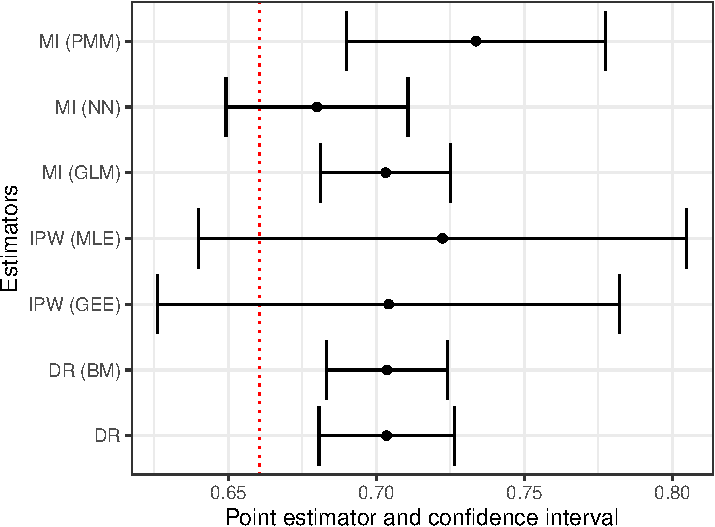
\includegraphics{nonprobsvy-paper_files/figure-latex/comparison-of-est-1} 

}

\caption[Comparison of estimates of the share of job vacancies offered on a single-shift]{Comparison of estimates of the share of job vacancies offered on a single-shift}\label{fig:comparison-of-est}
\end{figure}
\end{CodeChunk}

\subsection{Advanced usage}\label{advanced-usage}

\subsubsection{Bootstrap approach for variance
estimation}\label{bootstrap-approach-for-variance-estimation}

In the package we allow the user to estimate the variance of the mean
analytically (by default) or using the bootstrap approach, as described
in Section \ref{sec-prediction}. We use analytical variance estimators
proposed in the papers referenced in Section \ref{sec-methods}. The
calculation of the standard error can be disabled using
\code{nonprob(se=FALSE)}. The bootstrap approach implemented in the
package refers to:

\begin{itemize}
\item the non-probability sample -- currently only simple random sampling with replacement is available,
\item the probability sample -- all the approaches implemented in the \code{as.svrepdesign} function of the \pkg{survey} package are supported and we refer the reader to the relevant help file. 
\end{itemize}

The bootstrap approach is specified via the \code{control_inf()}
function with \texttt{var\_method\ =\ "bootstrap"}. The bootstrap method
for the probability sample is controlled via the \texttt{rep\_type}
argument, which passes the method to the \texttt{as.svrepdesign}
function. The number of iterations is set in the \texttt{num\_boot}
argument (100 by default). If the samples are large or the estimation
method is complicated (e.g.~involves variable selection) one can set
\texttt{verbose=TRUE} to track progress. By default bootstrap results
are stored in the \texttt{boot\_sample} element of the resulting list
(to disable this option, \texttt{keep\_boot} should be set to
\texttt{FALSE}). The following code is an example of applying the IPW
approach with the bootstrap approach specified by the argument
\texttt{control\_inference} of the \texttt{nonprob} function.

\begin{CodeChunk}
\begin{CodeInput}
R> ipw_est1_boot <- nonprob(
+   selection = ~ region + private + nace + size,
+   target = ~ single_shift,
+   svydesign = jvs_svy,
+   data = admin,
+   method_selection = "logit",
+   control_inference = control_inf(var_method = "bootstrap", num_boot = 50),
+   verbose = FALSE
+ )
\end{CodeInput}
\begin{CodeOutput}
Warning in ipw_maxlik(method, X_nons = X_nons, X_rand = X_rand, weights =
weights, : Warning in fitting selection model with the `maxLik` package:
probably not converged.
\end{CodeOutput}
\end{CodeChunk}

Next, we compare the estimated standard error of variance estimation for
the analytical and the bootstrap approach.

\begin{CodeChunk}
\begin{CodeInput}
R> rbind("IPW analytic variance"=ipw_est1$output,
+       "IPW bootstrap variance"=ipw_est1_boot$output)
\end{CodeInput}
\begin{CodeOutput}
                            mean         SE
IPW analytic variance  0.7223628 0.04207711
IPW bootstrap variance 0.7223628 0.04331885
\end{CodeOutput}
\end{CodeChunk}

The boot samples can be accessed via the \texttt{boot\_sample} element
of the output list of the \texttt{nonprob} function. Note that the
output is returned as a \texttt{matrix} because we allow multiple
\texttt{target} variables.

\begin{CodeChunk}
\begin{CodeInput}
R> head(ipw_est1_boot$boot_sample, n=3)
\end{CodeInput}
\begin{CodeOutput}
     single_shift
[1,]    0.6501353
[2,]    0.7887037
[3,]    0.7465485
\end{CodeOutput}
\end{CodeChunk}

\subsubsection{Variable selection
algorithms}\label{variable-selection-algorithms}

In this section we briefly show how to use variable selection
algorithms. In order to indicate that a variable selection algorithm
should be used one should specify the
\texttt{control\_inference\ =\ control\_inf(vars\_selection\ =\ TRUE)}
argument. Then, the user should either leave the default setting or
specify the outcome parameters via the \code{control_out} function or
the \code{control_sel} function. Both functions have the same
parameters:

\begin{itemize}
\item \code{penalty} -- The penalization function used during variables selection (possible values: \code{c("SCAD", "lasso", "MCP")})
\item \code{nlambda} -- The number of $\lambda$ values; by default set to 50.
\item \code{lambda_min} -- The smallest value for $\lambda$, as a fraction of \code{lambda.max}; .001 by default.
\item \code{lambda} -- A user specified vector of lambdas (only for the \code{control_sel} function).
\item \code{nfolds} -- The number of folds for cross validation; by default set to 10.
\item \code{a_SCAD, a_MCP} -- The tuning parameter of the SCAD and MCP penalty for the selection model; by default set to 3.7 and 3, respectively.
\end{itemize}

In the case of the MI approach we rely on the \pkg{ncvreg} package
\citep{ncvreg}, which is the only \proglang{R} package that employs the
SCAD method. For the IPW and DR approaches, we have developed our own
codes in \proglang{C++} via the \pkg{Rcpp} and \pkg{RcppArmadillo}
packages. In the code below we apply variable selection for the MI-GLM
estimator using only 5 folds, 25 possible values of \(\lambda\)
parameters and the LASSO penalty.

\begin{CodeChunk}
\begin{CodeInput}
R> mi_est1_sel <- nonprob(
+   outcome = single_shift ~ region + private + nace + size,
+   svydesign = jvs_svy,
+   data = admin,
+   method_outcome = "glm",
+   family_outcome = "binomial" ,
+   control_outcome = control_out(nfolds = 5, nlambda = 25, penalty = "lasso"),
+   control_inference = control_inf(vars_selection = TRUE),
+   verbose = TRUE
+ )
\end{CodeInput}
\begin{CodeOutput}
Starting CV fold #1
Starting CV fold #2
Starting CV fold #3
Starting CV fold #4
Starting CV fold #5
\end{CodeOutput}
\end{CodeChunk}

In this case study, the MI-GLM estimator with variable selection yields
almost the same results as the approach without it. Point estimates and
standard errors differ at the fourth and third digit, respectively.

\begin{CodeChunk}
\begin{CodeInput}
R> rbind("MI without var sel"=mi_est1$output,
+       "MI with var sel"=mi_est1_sel$output)
\end{CodeInput}
\begin{CodeOutput}
                        mean         SE
MI without var sel 0.7031991 0.01120162
MI with var sel    0.7019285 0.01102080
\end{CodeOutput}
\end{CodeChunk}

\section[Classes and S3Methods]{Classes and \code{S3Methods}}\label{sec-s3methods}

The package contains the main class \code{nonprobsvy} and a
supplementary class \code{summary_nonprobsvy}. All available
\code{S3methods} can be obtained by calling
\code{methods(class="nonprobsvy")}. For instance, the
\code{check_balance} function, already mentioned in the case study, is
used to view the balance by checking how the PS weights reproduce known
or estimated population totals; the \code{nobs} function returns the
sample size of the probability and non-probability samples:

\begin{CodeChunk}
\begin{CodeInput}
R> nobs(dr_est1)
\end{CodeInput}
\begin{CodeOutput}
   prob nonprob 
   6523    9344 
\end{CodeOutput}
\end{CodeChunk}

Table \ref{tab-s3methods} presents methods implemented for the
\code{nonprobsy} class. On purpose we did not implement many methods as
the goal of the package is to provide point and interval estimates. If a
user is interested in assessing the quality of the models or covariate
balance should use existing \proglang{R} packages.

\begin{table}[ht!]
\centering
\small
\begin{tabular}{p{4cm}p{11cm}}
\hline 
Function & Description \\
\hline
\code{check_balance} & aaa; \\
\code{confint} & aaa\\
\code{nobs} & \\
\code{pop_size} & \\
\code{summary} & \\
\code{logLik, AIC, BIC, deviance} & \\
\code{residuals, hatvalues, cooks.distance, print, vcov}  & it works exactly like \code{glm} counterparts.\\
\hline 
\end{tabular}
\caption{\code{S3Methods} implemented in the \pkg{nonprobsvy}}
\label{tab-s3methods}
\end{table}

\section{Summary and future work}\label{summary-and-future-work}

The \pkg{nonprobsvy} package provides a comprehensive \proglang{R}
software solution that addresses inference challenges connected with
non-probability samples by integrating them with probability samples or
known population totals/means. As non-probability data sources like
administrative registers, voluntary online panels, and social media data
become increasingly available, statisticians need robust methods to
produce reliable population estimates. The package implements
\textit{state-of-the-art} approaches including mass imputation, inverse
probability weighting, and doubly robust methods, each designed to
correct selection bias by leveraging auxiliary data. By providing a
unified framework and its integration with the \pkg{survey} package, the
\pkg{nonprobsvy} makes complex statistical methods for non-probability
samples more accessible, enabling researchers to produce robust
estimates even when working with non-representative data.

There are several avenues for future development of the \pkg{nonprobsvy}
package. One key priority is to implement model-based calibration and
additional methods for estimating propensity scores and weights. The
package currently assumes no overlap between probability and
non-probability samples, so accounting for potential overlap (e.g., in
big data sources and registers) is another important extension.
Additional planned developments include handling non-ignorable sample
selection mechanisms, developing a theory for maintaining consistency
with calibration weights, and supporting multiple non-probability
samples from various sources for the purpose of data integration.
Further methodological extensions under consideration include empirical
likelihood approaches for doubly/multiply robust estimation, integration
of machine learning methods like debiased/double machine learning from
causal inference, handling measurement errors in big data variables, and
expanding the bootstrap approach beyond simple random sampling with
replacement.

The package will also be extended to handle the \texttt{svyrep.design}
class from the \pkg{survey} package and the \pkg{svrep} package. These
developments will enhance its capabilities for handling complex survey
data structures and modern estimation challenges.

\section{Acknowledgements}\label{sec-acknowledgements}

The authors' work has been financed by the National Science Centre in
Poland, OPUS 20, grant no. 2020/39/B/HS4/00941.

Łukasz Chrostowski is the main developer and maintainer of the package
up to version 0.1.0. Parts of this work are based on Łukasz's master's
thesis (available at
\url{https://github.com/ncn-foreigners/graduation-theses}). Piotr
Chlebicki contributed to the package and implemented the MI-PMM
estimators. Maciej Beręsewicz had the initial idea and was responsible
for the design of the package, as well as testing, reviewing and
contributing to the source code and preparing the manuscript. He was
also responsible for the major restructuring of the package between
0.1.0 and 0.2.0 and subsequent releases.

\clearpage

\appendix

\section{List of symbols}\label{list-of-symbols}

\begin{table}[ht!]
\centering
\begin{tabular}{ll}
\hline
\textbf{Symbol} & \textbf{Description} \\
\hline
$U$ & Target population of size $N$ \\
$S_A$ & Non-probability sample \\
$S_B$ & Probability sample \\
$N$ & Population size \\
$n_A$ & Size of non-probability sample \\
$n_B$ & Size of probability sample \\
$\hat{N}^A$ & Estimated size based on non-probability sample \\
$\hat{N}^B$ & Estimated size based on probability sample \\
$\boldsymbol{x}_i$ & Vector of auxiliary variables for unit $i$ \\
$y_i$ & Value of the study/target variable for unit $i$ \\
$y_i^*$ & Imputed value for unit $i$ in $S_B$\\
$\pi_i^A$ & Propensity score for unit $i$ in non-probability sample \\
$\pi_i^B$ & Inclusion probability for unit $i$ in probability sample \\
$d_i^A$ & Inverse probability weight ($1/\pi_i^A$) for non-probability sample \\
$d_i^B$ & Design weight ($1/\pi_i^B$) for probability sample \\
$R_i^A$ & Indicator of inclusion into non-probability sample \\
$R_i^B$ & Indicator of inclusion into probability sample \\
$\mu$ & Population mean of target variable $y$ \\
$\mu_{\boldsymbol{x}}$ & Population means of auxiliary variables $\boldsymbol{x}$ \\
$m(\boldsymbol{x}_i, \boldsymbol{\beta})$ & Semiparametric model for outcome variable \\
$\dot{m}(\boldsymbol{x}_i, \boldsymbol{\beta})$ & First derivative of the $m(\boldsymbol{x}_i, \boldsymbol{\beta})$ with respect to $\boldsymbol{\beta}$ \\
$\pi(\boldsymbol{x}_i, \boldsymbol{\gamma})$ & Propensity score model for $R_i^A$ \\
$\boldsymbol{\beta}$ & Parameter vector for outcome model \\
$\boldsymbol{\gamma}$ & Parameter vector for propensity score model \\
$\lambda_{\boldsymbol{\beta}}, \lambda_{\boldsymbol{\gamma}}$ & Tuning parameters for penalisation methods \\
$\hat{\mu}_{\boldsymbol{x}}$ & Estimator for the population means of auxiliary variables $\boldsymbol{x}$ \\
$\bar{\boldsymbol{x}}_{A}$ & A vector of the sample means of the auxiliary variables $\boldsymbol{x}$ from $S_A$ \\ 
$\hat{\mu}_{PR}$ & Prediction estimators \\
$\hat{\mu}_{MI}$ & Mass imputation estimator \\
$\hat{\mu}_{IPW}$ & Inverse probability weighting estimator \\
$\hat{\mu}_{DR}$ & Doubly robust estimator \\
$\hat{V}_{boot}$ & Variance estimator based on the bootstrap \\
\hline
\end{tabular}
\caption{List of symbols and their descriptions}
\label{tab-list-of-symbols}
\end{table}

\clearpage

\section{Algorithms for the MI-NN and MI-PMM
estimators}\label{sec-details}

\begin{algorithm}[ht!]
\caption{Mass imputation using the $k$ nearest neighbour algorithm}
\label{algo-2}
\begin{algorithmic}[1]
\State If $k=1$, then for each $i \in S_B$ match $\hat{\nu}(i)$ such that
$\displaystyle \hat{\nu}(i)=
\operatornamewithlimits{arg\,min}_{j\in S_{A}}d\left(\boldsymbol{x}_i,\boldsymbol{x}_j\right)$.
\State If $k>1$, then
$$\hat{\nu}(i, z) = \operatornamewithlimits{arg\,min}_{\displaystyle j\in S_{A}\setminus\bigcup_{t=1}^{z-1}
\{\hat{\nu}(i, t)\}} d\left(\boldsymbol{x}_i, \boldsymbol{x}_j\right)$$
i.e. $\hat{\nu}(i, z)$ is $z$-th nearest neighbour from the sample $S_A$.\;
\State For each $i \in S_B$, calculate the imputed value as

$$
y_i^* = \frac{1}{k}\sum_{t=1}^{k}y_{\hat{\nu}(i, t)}.
$$
\end{algorithmic}
\end{algorithm}

\begin{algorithm}[ht!]
\caption{Mass imputation using predictive mean matching variant: $\hat{y}-\hat{y}$ matching}
\label{algo-3}
\begin{algorithmic}[1]
\State Estimate regression model $m(\boldsymbol{x}, \boldsymbol{\beta})$ parameters.\;
\State Predict 

$$\hat{y}_{i}=m\left(\boldsymbol{x}_{i},\hat{\boldsymbol{\beta}}\right),  \hat{y}_{j}=m\left(\boldsymbol{x}_{j},\hat{\boldsymbol{\beta}}\right)$$

for $i\in S_{B}, j\in S_{A}$ and assign each  $i\in S_{B}$ to $\hat{\nu}(i)$, where

$$
\displaystyle \hat{\nu}(i)=
\operatornamewithlimits{arg\,min}_{j\in S_{A}}d\left(\hat{y}_{i},\hat{y}_{j}\right).
$$ 

\State If $k>1$, then:
$$
\hat{\nu}(i, z) = \operatornamewithlimits{arg\,min}_{\displaystyle j\in S_{A}\setminus\bigcup_{t=1}^{z-1}
\{\hat{\nu}(i, t)\}} d\left(\hat{y}_{i},\hat{y}_{j}\right)
$$
e.g., $\hat{\nu}(i, z)$ is $z$-th nearest neighbour from a sample $S_A$.\;
\State For $i \in S_B$, calculate imputation value as 
$$
y_i^* = \frac{1}{k}\sum_{t=1}^{k}y_{\hat{\nu}(i, t)}.
$$
\end{algorithmic}
\end{algorithm}

\begin{algorithm}[ht!]
\caption{Mass imputation using predictive mean matching variant: $\hat{y}-y$ matching}
\label{algo-4}
\begin{algorithmic}[1]

\State Estimate regression model $m(\boldsymbol{x}, \boldsymbol{\beta})$ parameters.\;

\State Predict 
$$
\hat{y}_{i}=m\left(\boldsymbol{x}_{i},\hat{\boldsymbol{\beta}}\right)
$$  for $i \in S_{B}$ 
and assign each  $i \in S_{B}$ do $\hat{\nu}(i)$, where
$$
\displaystyle \hat{\nu}(i)=
\operatornamewithlimits{arg\,min}_{j \in S_{A}}d\left(\hat{y}_{i},y_{j}\right)
$$.\;
\State If $k>1$, then:
$$
\hat{\nu}(i, z) = \operatornamewithlimits{arg\,min}_{\displaystyle j \in S_{A} \setminus \bigcup_{t=1}^{z-1}
\{\hat{\nu}(i, t)\}} d\left(\hat{y}_{i},y_{j}\right).
$$
\State For each $i \in S_B$ calculate imputation value as
$$
y_i^* = \frac{1}{k}\sum_{t=1}^{k}y_{\hat{\nu}(i, t)}.
$$
\end{algorithmic}
\end{algorithm}

\newpage

\bibliography{references.bib}



\end{document}
